\documentclass[12pt]{article}
\usepackage[utf8]{inputenc}
\usepackage[english]{babel}
\usepackage{listings}
\usepackage{tikz}
\tikzset{main node/.style={circle,fill=white!20,draw,minimum size=1cm,inner sep=0pt},}
\usepackage{verbatim}
\newcommand{\HRule}{\rule{\linewidth}{0.5mm}}

\begin{document}

\begin{center}
\textsc{\LARGE Principles of Computer System Design}\\[0.3cm] % Context
\HRule \\[0.4cm]
{ \huge \bfseries Assignment 2} % Main title
\HRule \\[0.4cm]
\large
Johannes de Fine Licht % Names
\\Philip Graae
\\Ola Rønning
\\\today
\end{center}

\section*{Question 1: Serializability \& Locking} % Question 1

\subsection*{Schedule 1}
\begin{figure}[h!]
\texttt{T1: R(X)\hspace{250pt}W(Y) C\\
T2:\hspace{50pt}W(Z) W(X) C \\
T3:\hspace{150pt}R(Z) R(Y) C}
\caption{Schedule one.}
\label{sch1}
\end{figure}
Schedule one, reproduced above, correspondence to the precedence graph in figure~\ref{p1}.
\begin{figure}[h!]
\centering
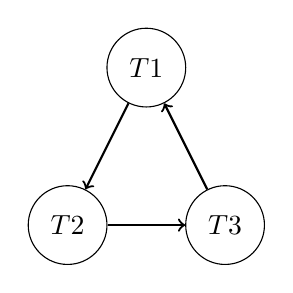
\begin{tikzpicture}
    \node[main node] (1) at (0,1)      {$T1$};
    \node[main node] (2) at (-1, -1) {$T2$};
    \node[main node] (3) at (1, -1)  {$T3$};

    \path[draw,thick,->]
    (1) edge node {} (2)
    (2) edge node {} (3)
    (3) edge node {} (1);
\end{tikzpicture}
\caption{Precedence graph for Schedule one, see figure~\ref{sch1}.}
\label{p1}
\end{figure}
The precedence graph, see figure~\ref{p1}, contains a cycle between transactions: \texttt{T1,T2,T3} and is hence not conflict serializable. As schedulers using Strict two phase locking allows only conflict serializable schedules. Schedule one is not conflict serializable and therefore cannot have been produced by a scheduler following Strict two phase locking.
\subsection*{Schedule 2} 
\begin{figure}[h!]
\texttt{T1: R(X)\hspace{150pt}W(Y) C\\
T2:\hspace{130pt}R(Z)\hspace{120pt}W(X) W(Y) C\\
T3:\hspace{50pt}W(Z) C}
\caption{Schedule two.}
\label{sch2}
\end{figure}
Schedule two, reproduced above, correspondence to the precedence graph in figure~\ref{p2}.
\begin{figure}[h!]
\centering
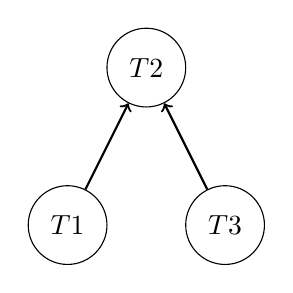
\begin{tikzpicture}
    \node[main node] (2) at (0,1)    {$T2$};
    \node[main node] (1) at (-1, -1) {$T1$};
    \node[main node] (3) at (1, -1)  {$T3$};

    \path[draw,thick,->]
    (1) edge node {} (2)
    (3) edge node {} (2);
\end{tikzpicture}
\caption{Precedence graph for Schedule one, see figure~\ref{sch2}.}
\label{p2}
\end{figure}
The precedence graph, see figure~\ref{p2}, is acyclic and hence is conflict serializable. In particular schedule two, is equivalent with a serial schedule where transaction two is performed last. As schedule 2 is conflict serializable, schedule 2 could be scheduled by a scheduler following Strict two phase locking. The injection of shared and exclusive locks required if the scheduler was using Strict two phase locking is reproduced below, figure~\ref{locks}.
\begin{figure}[h!]
\texttt{T1: S(X)\hspace{95pt}E(Y)RS(X)RE(Y)\\
T2:\hspace{105pt}S(Z)\hspace{90pt}E(X)E(Y)RS(Z)RE(X)RE(Y)\\
T3:\hspace{50pt}E(Z)RE(Z)}
\label{locks}
\caption{Shared and exclusive locks that need to be acquired in order for schedule two, see figure~\ref{sch2}, to be scheduled using Strict two phase locking. \texttt{S(Q)} acquires a shared lock on \texttt{Q} and \texttt{RS(Q)} releases the lock on \texttt{Q}, exclusive locks follow the same semantics, only with an \texttt{E}.}
\end{figure}
\section*{Question 2: Optimistic Concurrency Control}
\subsection*{Scenario 1}
\begin{figure}[h!]
\texttt{T1: RS(T1) = \{1, 2, 3\}, WS(T1) = \{3\},\\
T1 completes before T3 starts.\\
T2: RS(T2) = \{2, 3, 4\}, WS(T2) = \{4, 5\},\\
T2 completes before T3 begins with its write phase.\\
T3: RS(T3) = \{3, 4, 6\}, WS(T3) = \{3\},\\
allow commit or rollback?}
\end{figure}
\subsection*{Scenario 2}
\begin{figure}[h!]
\texttt{T1: RS(T1) = \{2, 3, 4, 5\}, WS(T1) = \{4\},\\
T1 completes before T3 begins with its write phase.\\
T2: RS(T2) = \{6, 7, 8\}, WS(T2) = \{6\},\\
T2 completes read phase before T3 does.\\
T3: RS(T3) = \{2, 3, 5, 7, 8\}, WS(T3) = \{7, 8\},\\
allow commit or rollback?}
\end{figure}
\subsection*{Scenario 3}
\begin{figure}[h!]
\texttt{T1: RS(T1) = \{2, 3, 4, 5\}, WS(T1) = \{4\},\\
T1 completes before T3 begins with its write phase.\\
T2: RS(T2) = \{6, 7, 8\}, WS(T2) = \{6\},\\
T2 completes before T3 begins with its write phase.\\
T3: RS(T3) = \{2, 3, 5, 7, 8\}, WS(T3) = \{7, 8\},\\
allow commit or rollback?}
\end{figure}
\section*{Programming Task}
\section*{Questions for Discussion on Architecture} % Question 3
\subsection*{1.} % Question 3.1
\subsection*{2.} % Question 3.2
\subsection*{3.} % Question 3.3
\subsection*{4.} % Question 3.4
\end{document}
